\documentclass[11pt, hidelinks, a4paper]{scrartcl}
    \usepackage{amsmath,amssymb}
    \usepackage{booktabs}  % For \toptrule etc.
    \usepackage{authblk}  % For author/affiliation compilation.
    \usepackage{caption}
        \captionsetup{parskip=10pt, margin=0.5cm}
        \captionsetup{font=footnotesize}
    \usepackage{comment}
    \usepackage[top=30truemm,bottom=35truemm,left=30truemm,right=30truemm]{geometry}
    \usepackage{graphicx}
    \usepackage{hyperref}
    % \usepackage{lineno}\linenumbers
    \usepackage{multicol}
    \usepackage[section]{placeins} % For per-chapter float placings. Package also provides \FloatBarrier.
    \usepackage{xspace}

    \newcommand{\tn}[1]{\textnormal{#1}}
    \newcommand{\eV}{\text{e\kern-0.15ex V}\xspace}
    \newcommand{\GeV}{\text{G\eV}\xspace}
\graphicspath{{img_proceedings/}}

\title{\textbf{A combined fit to the Higgs Branching Ratios at ILD} }
\author{Jonas~Kunath\thanks{Presenter.
    Talk presented at the International Workshop on Future Linear Colliders (LCWS2021),
    15-18 March 2021. C21-03-15.1}
}
\author{Fabricio~Jimenez~Morales}
\author{Jean-Claude~Brient}
\author{Vincent~Boudry}
\affil{Laboratoire Leprince-Ringuet CNRS, \'Ecole Polytechnique,\hspace{2em} Institut Polytechnique de Paris, France}
%
\date{}
\begin{document}
\maketitle
\begin{abstract}
Higgs decay branching ratios at a future Higgs factories
can be measured by directly exploiting class numeration.
Given the clean environment at a lepton collider,
it is possible to build an event sample highly enriched in Higgs bosons
and essentially unbiased for any decay mode.
The sample can be partitioned into categories using event properties
linked to the expected Higgs decay modes.
The counts per category are used to fit
the Higgs branching ratios in a model independent way.
The result of the fit is directly the set of branching ratios,
independent from any measurement of a Higgs production mode.

We present a simplified study on simulated data
for the International Linear Detector (ILD)
at the International Linear Collider (ILC) at 250~\GeV.
\end{abstract}

\section{Introduction}
A Higgs factory will produce a large number of Higgs bosons
in the comparatively simple collision environment of a lepton collider.
The projected gain on the precision of measurements of the particle's parameters
will make these measurements sensitive to deviations
that are predicted by theories of physics beyond the Standard Model.
Multiple proposals exist for Higgs factories operating at a center-of-mass energy
close to the peak of the Higgsstrahlung production cross section,
$\sqrt{s}\approx250~\GeV$.

With the Higgsstrahlung process at a Higgs factory
it is possible to construct an unbiased sample
in which each type of Higgs decay occurs with the probability given by
its branching ratio (BR) realized in nature~\cite{HiggsBR_LCWS2019}.
Higgsstrahlung events with $Z \to e^+ e^-$ and $Z \to \mu^+ \mu^-$
can be selected through
the Z boson, independent of the Higgs decay \cite{hRecoilIndependence}.

Figure~\ref{fig:toys} (left) shows how such a sample can be partitioned
into a number of classes with each of the class selection efficiencies depending
on the specific Higgs decay mode.
The relative frequency of the number of events per class
depends on the Higgs BRs.
An inclusive estimation of all branching ratios can be obtained
through a fit on the class counts.
The approach naturally lends itself to an extension with additional classes
which target a beyond Standard Model Higgs decay.
Additional decay modes can thus be excluded
with an upper limit related to the sample size.

The presented study is realized in the context of the
International Linear Detector (ILD)~\cite{ILD_DBD,ILD_IDR}.
The ILD detector concept is proposed for the International Linear Collider (ILC).
The detector design is based on the particle flow approach
for particle reconstruction~\cite{ParticleFlow}.
Only running scenarios of the ILC
with a center-of-mass energy of $\sqrt{s}=250~\GeV$ (ILC250)
are considered here.

The fit is in a preliminary state.
The simulation procedure is described in section~\ref{sec:simulation},
a summary of the
current simplifications in~\ref{subsec:simplifications}.
Preliminary results from the fit,
with some known shortcomings, are already available.
They are given in section~\ref{sec:fit}.
An outline of the necessary future work is presented
in section~\ref{sec:future_work}.
Finally, the note is summarized in section~\ref{sec:conclusion}.

\section{Simulation}\label{sec:simulation}
We use samples produced by the ILD concept group since 2020.
They are obtained from a detailed simulation of the ILC250
with the new SetA beam parameters~\cite{ILC_Staging_2017}.

The events are generated at leading order using
WHIZARD version 2.8.5~\cite{whizard,omega}.
Initial State Radiation, Beamstrahlung and Final State Radiation are included.
The fragmentation and hadronization of final-state quarks and gluons
is performed with PYTHIA 6.422~\cite{pythia}.
The ILD detector geometry is described with DD4hep~\cite{DD4hep}
and simulated in GEANT4~\cite{GEANT4}.
Event reconstruction is performed with ILCSoft v02-02~\cite{ILCSoft},
which includes PandoraPFA~\cite{PandoraPFA} for
the construction of particle flow objects
and LCFIPlus~\cite{LCFIPlus} for flavor tagging.

\subsection{Current simplifications}\label{subsec:simplifications}
Results shown here are obtained without considering background processes.
As signal channel, $\nu \bar{\nu} H$ is used without a pre-selection step.
While it is not a realistic scenario,
this pure-Higgs sample can provide a first idea
of the precision and adaptability of the method.

For each of the nine considered main BRs of the Higgs boson,
at least 400k simulated events are used.
They are separately weighted and combined into a single sample
with exactly 40k signal Higgs events.
Different Higgs BR scenarios are tested by changing the weights.

Note that 40k Higgs events corresponds to about 10\% of the Higgs bosons
produced in the long-running H-20 scenario of the ILC250~\cite{ILC_Scenarios}.
Even before taking into account selection inefficiencies
only less than 7\% of the produced Higgs bosons
are in the $Z \to e^+ e^-$ and $Z \to \mu^+ \mu^-$ samples combined.
As mentioned in section \ref{sec:future_work}
we expect to be able to leverage the $\nu \bar{\nu} H$ sample.
Future work will have to show if a 10\% sample size
is a good estimation of the gain from the $\nu \bar{\nu} H$ sample.

\section{Branching ratio uncertainties}\label{sec:fit}
For each Higgs decay mode, a probability vector is
constructed from the simulation.
This vector stores the selection efficiency and the probability
for the events from the chosen type to fall into each of the classes
that are constructed within the sample.
The vectors can be collected as columns into a probability matrix $M$.
% The expected background counts per class have to be calculated as well.

An equivalent but statistically independent test sample (MC2) is used as an input for
the data counts per class.
To evaluate the adaptability of the fit, the Higgs BRs in MC2
can be altered, or new decay modes can be added.

A fit is then performed with \texttt{iminuit}~\cite{Minuit,iminuit}.
The Standard Model (SM) Higgs branching ratios (BRs)
are taken
as the starting values of the fit.
Based on a multinomial log-likelihood as its cost function,
the 9 considered independent BRs of the Higgs boson
are described through 8 parameters in the fit.
We obtain a prediction for the 8 parameters
and the corresponding covariance matrix.
From those we get the mean values and uncertainties for the BRs.

The result of this fit is shown in figure~\ref{fig:brs} for
the SM BRs and an alternative scenario.
Since the probability vectors of the decay modes are different enough,
the fit moves to the altered BRs without any problems.
The fit not landing at the altered BRs
would have suggested that the defined classes
do not have sufficient discriminating power
between some of the BRs.

The uncertainties on the BRs can be tested in a toy study.
The uncertainties and correlations of the fit on the expected event counts
are obtained through the second derivatives of the likelihood function
at the fit optimum.
For the toy study, samples are drawn from a multinomial distribution centered on the
expected counts for each class.
Then, a fit is performed for each of the samples, and the predicted
branching ratio optima are collected.
An example toy study on the $H \to b \bar{b}$ branching ratio is shown in
figure~\ref{fig:toys} (right).
The values from the toy study agree well with those anticipated
from the fit on the expected event counts.

The projected (absolute) $1 \sigma$-uncertainties for the Higgs branching ratios
are listed in table~\ref{tab:br_uncertainties}.
The numbers are based on the simplified scenario
outlined in section~\ref{subsec:simplifications}.

\begin{figure}[ht]
    \centering
    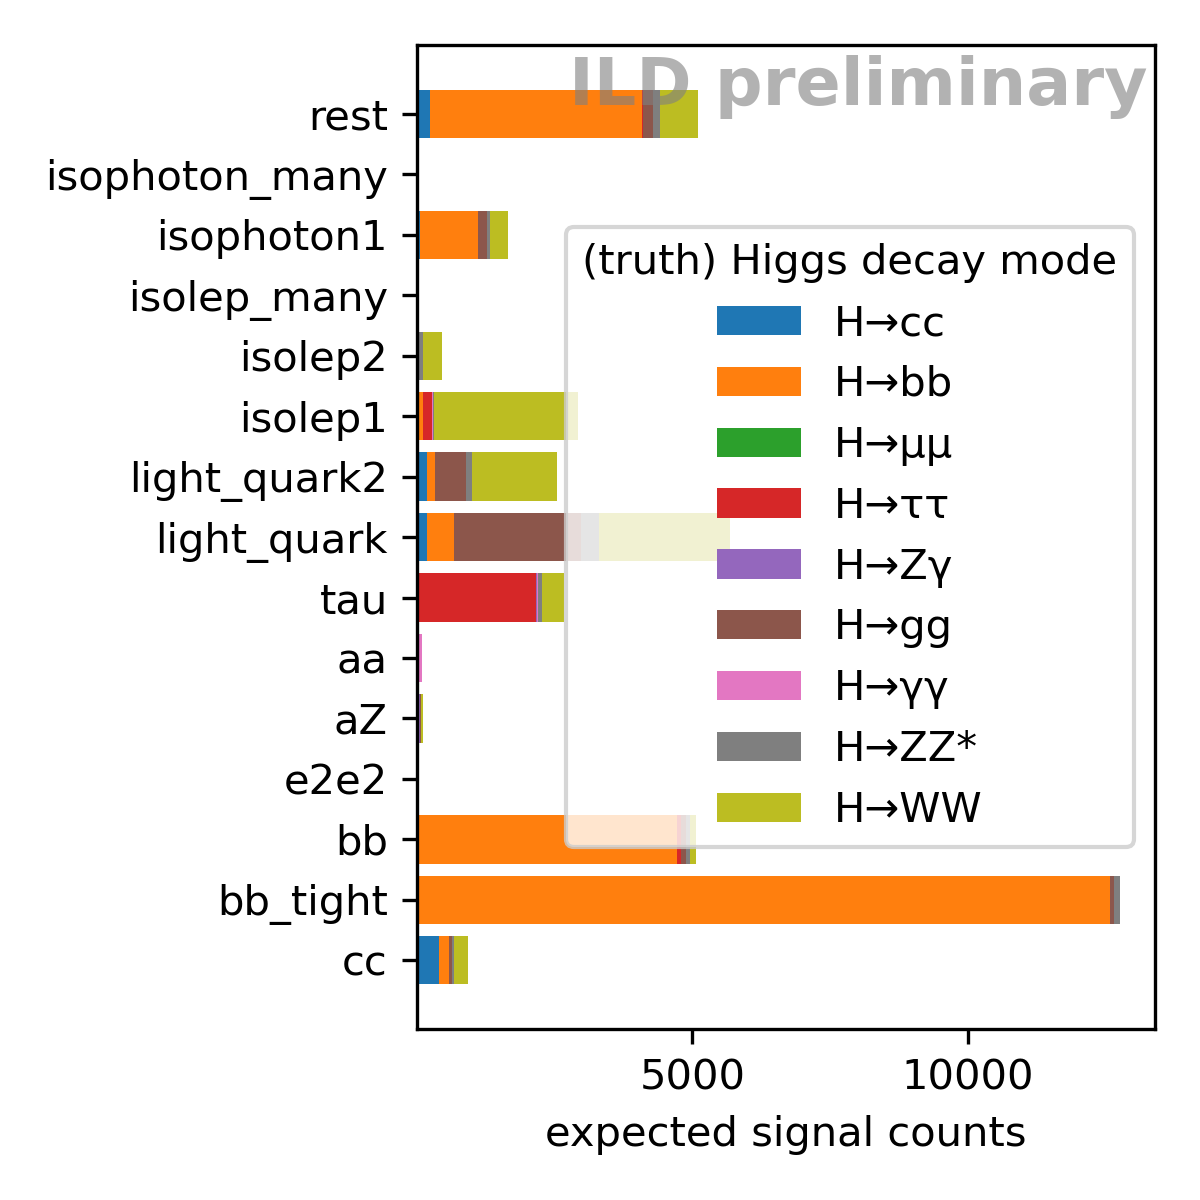
\includegraphics[width=0.49\textwidth, keepaspectratio]{intro_category_counts}
    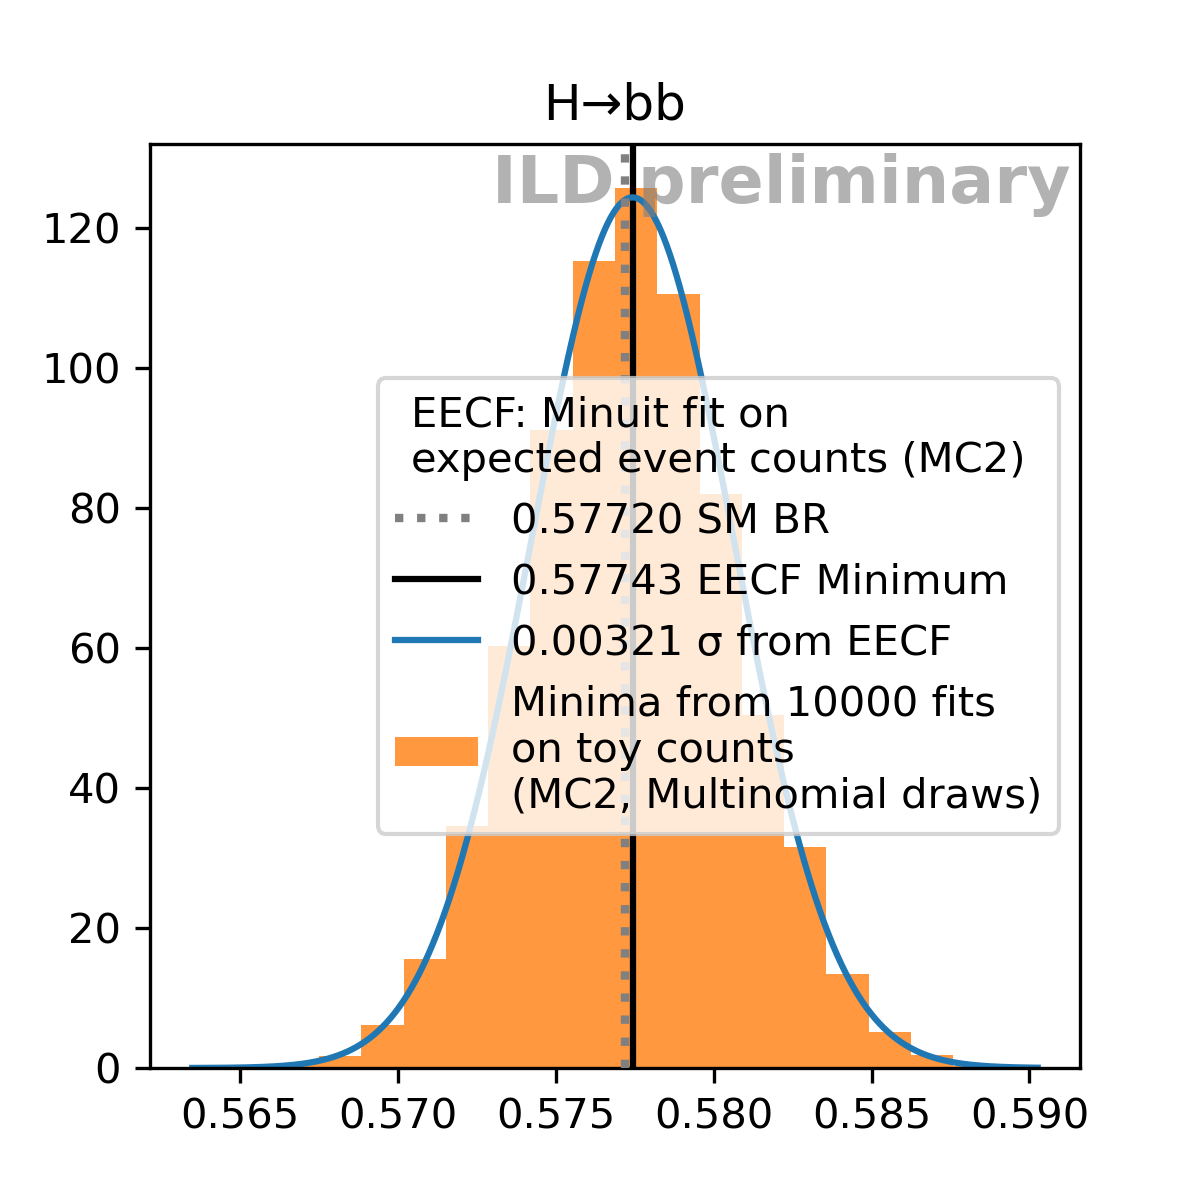
\includegraphics[width=0.49\textwidth, keepaspectratio]{H_bb}
    \caption{
        Left: Expected contributions per class from each of the Higgs decay modes
        assuming the Standard Model branching ratios.
        The class definitions are listed in the appendix.
        \\
        Right: Validation of the uncertainty from
        a fit on the expected event counts scenario against a toy study.
        The dotted grey line indicates the SM value of
        the $H \to b \bar{b}$ coupling in the simulation.
        The black line indicates the optimum of a fit on
        the expected event counts.
        It was validated that the difference between these two lines
        is only due to limited Monte Carlo statistics.
        The blue gaussian curve has as standard deviation the uncertainty of
        the fit on the expected event counts, as quoted by \texttt{MINUIT}.
        The orange histogram contains the fit optima from
        10k fits on event counts varied according to
        a multinomial distribution centered on the expected event counts.
    }\label{fig:toys}
\end{figure}

\begin{figure}[ht]
    \centering
    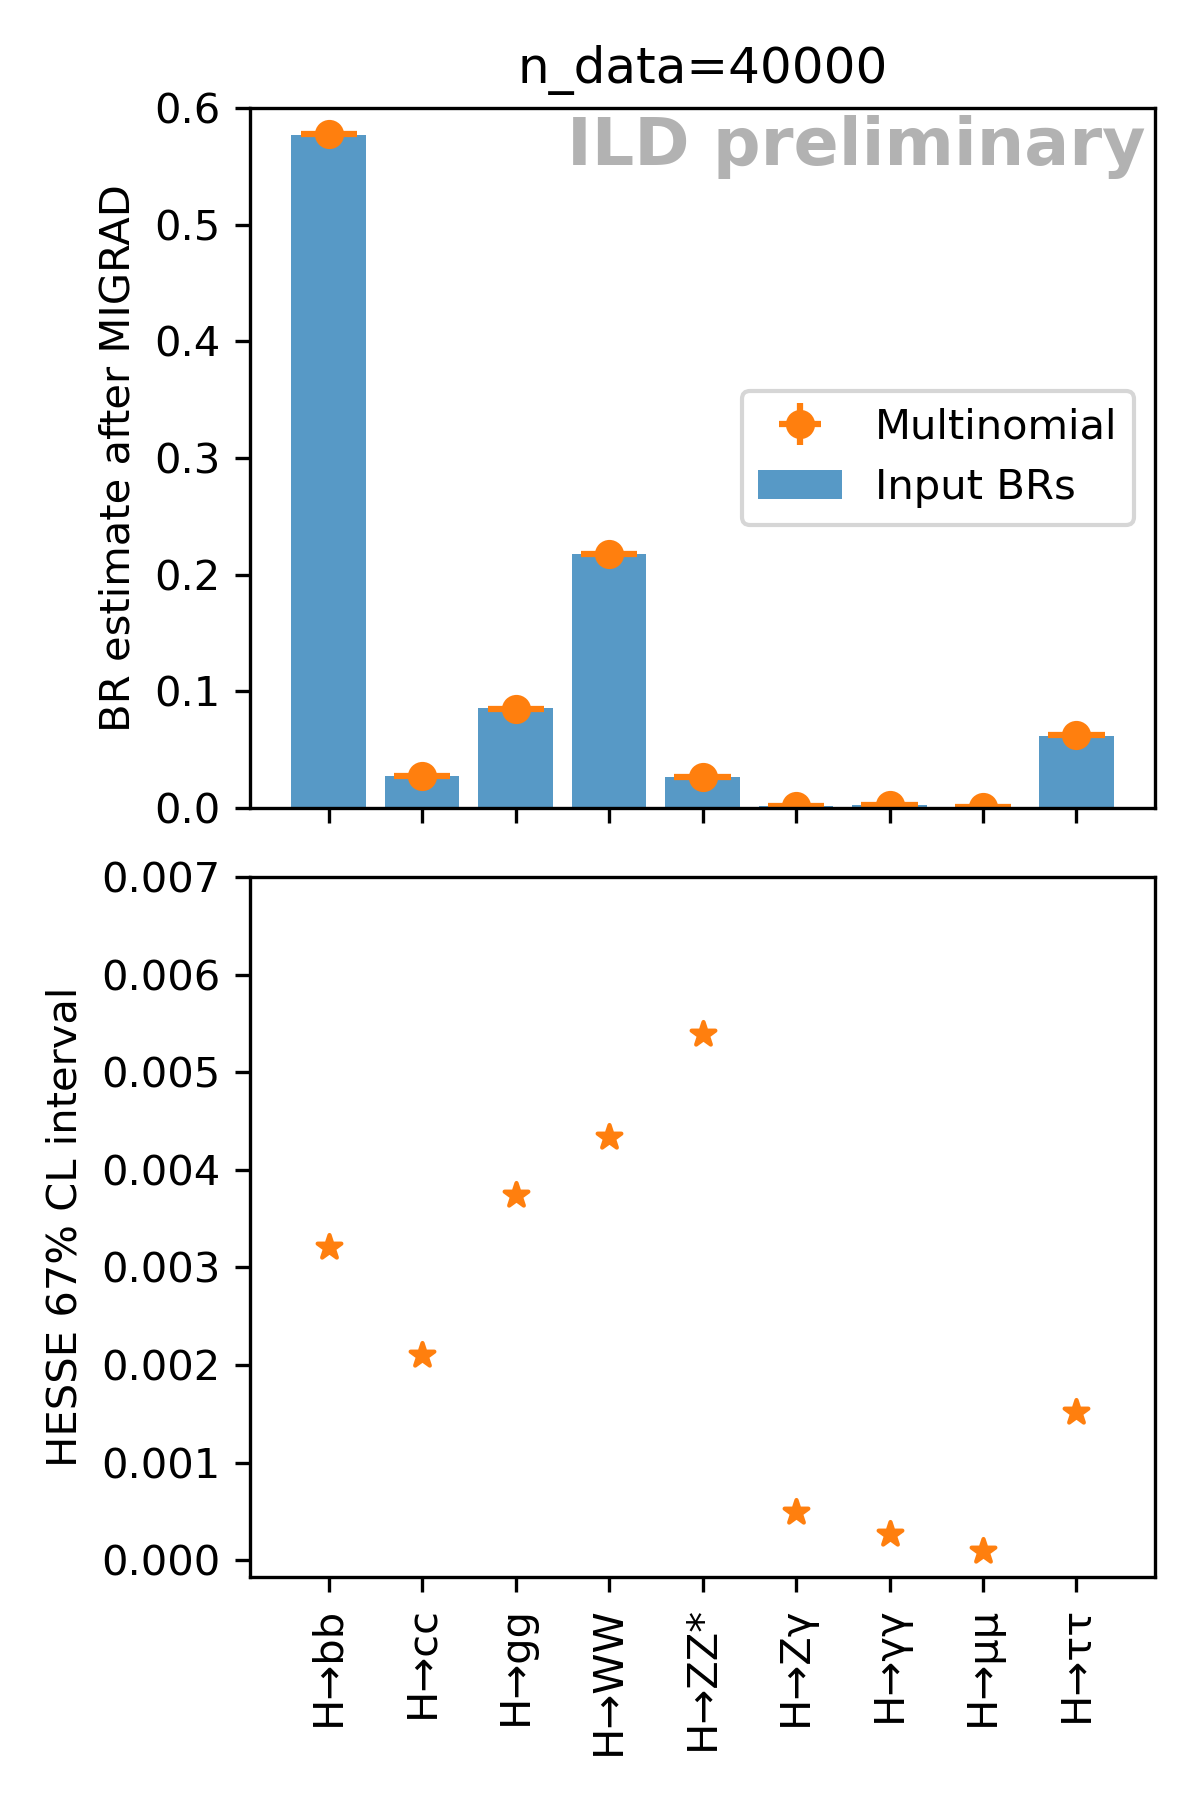
\includegraphics[width=0.49\textwidth, keepaspectratio]{br_estimates}
    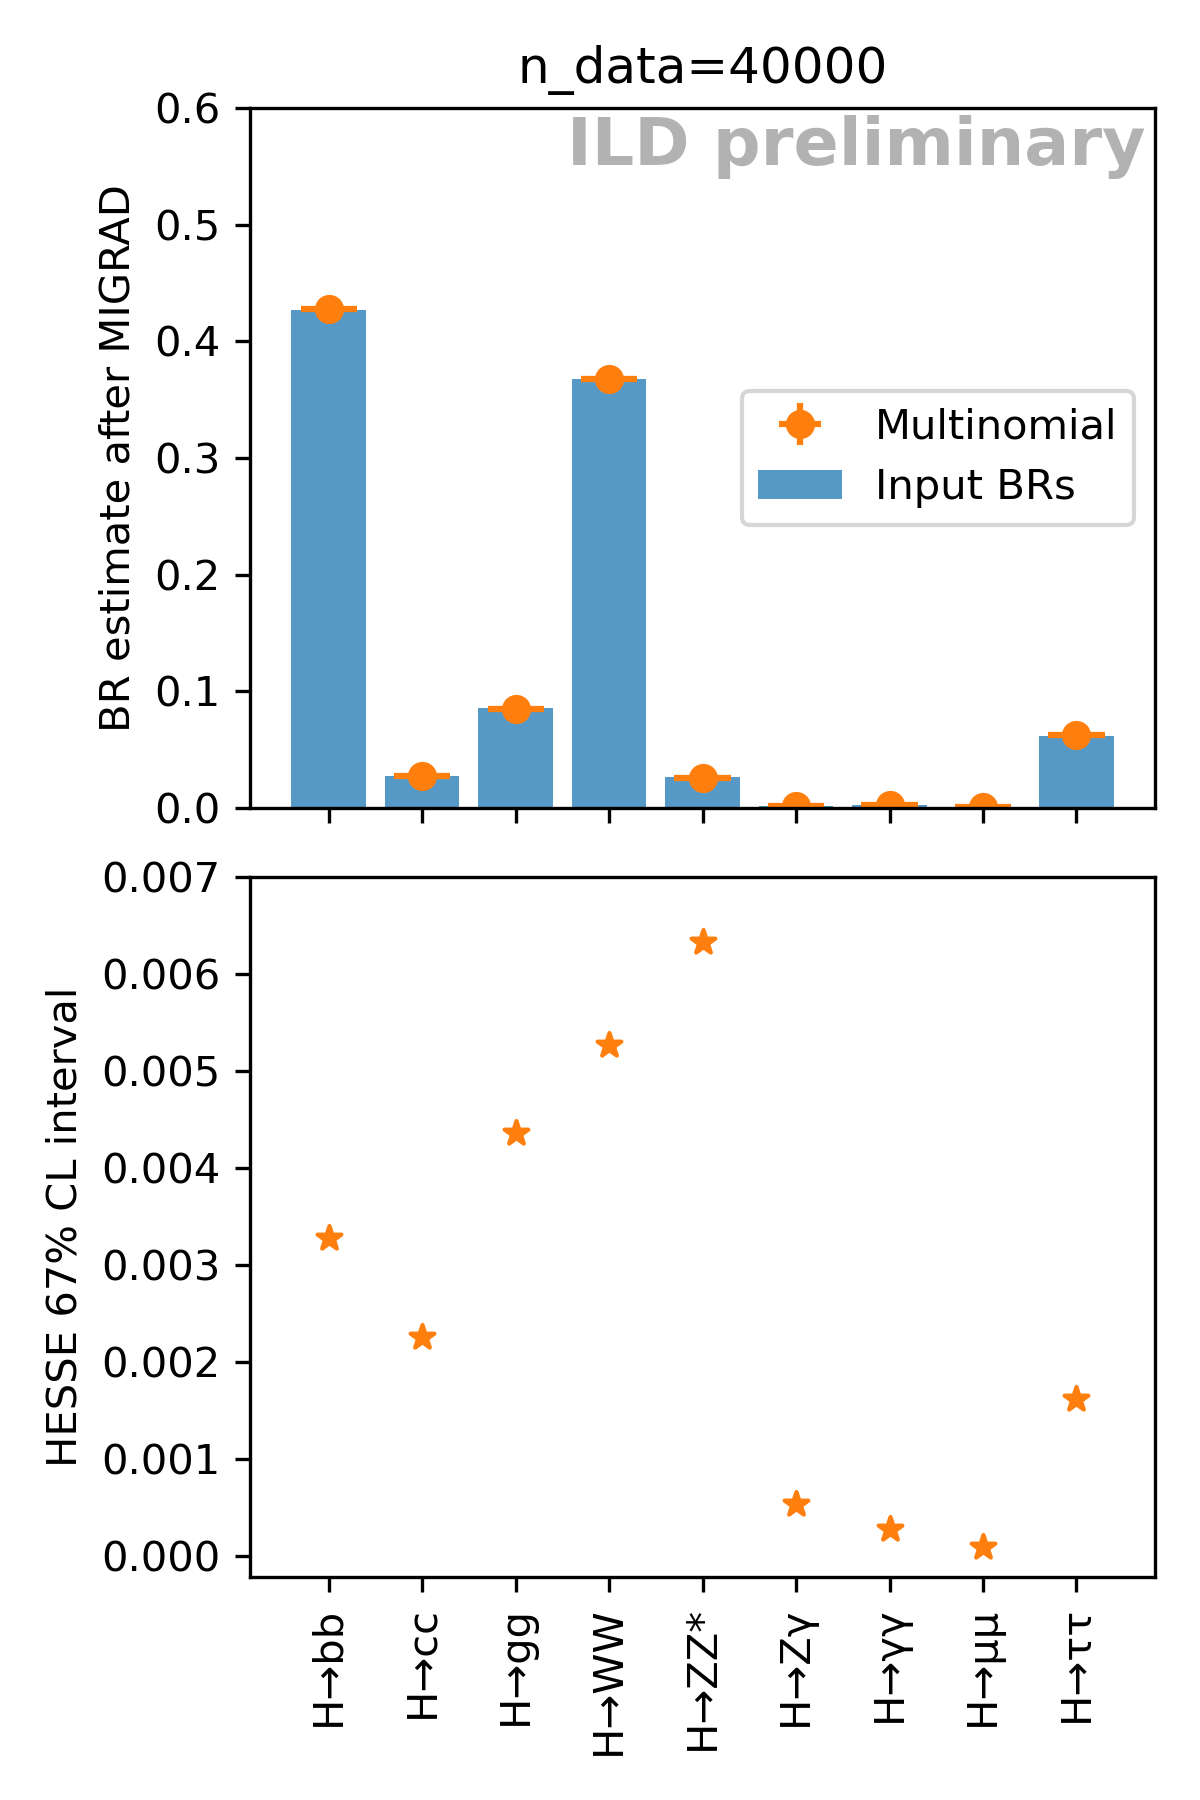
\includegraphics[width=0.49\textwidth, keepaspectratio]{changed_br_estimates}
    \caption{
        Top row: Branching ratios assumed for the generation of the counts per class.
        Fit optimum and its uncertainty as orange error bars.
        The starting values of the fit are
        the SM Higgs BRs for both cases.
        \\
        Bottom row: The absolute statistical fit uncertainties per branching ratio.
        \\
        Left: SM BRs.
        \\
        Right: The Higgs BRs in the simulation are the SM values
        with the changes
        $BR(H \to b \bar{b}) \searrow 15\%$, $BR(H \to W^+W^-) \nearrow 15\%$.
        The fit is able to move to the new minimum.
    }\label{fig:brs}
\end{figure}

\begin{table}[ht]
    \centering
    \begin{tabular}{lrrr}
        \toprule
        {} &  SM BR &  fitted BR &  $\sigma_{\tn{stat}}$ \\
        \midrule
        $H\to cc$           &  2.718 &    2.733 &     0.210 \\
        $H\to bb$           & 57.720 &   57.743 &     0.321 \\
        $H\to \mu\mu$       &  0.030 &    0.030 &     0.009 \\
        $H\to \tau\tau$     &  6.198 &    6.207 &     0.152 \\
        $H\to Z\gamma$      &  0.170 &    0.176 &     0.050 \\
        $H\to gg$           &  8.550 &    8.499 &     0.374 \\
        $H\to \gamma\gamma$ &  0.242 &    0.243 &     0.027 \\
        $H\to WW$           & 21.756 &   21.761 &     0.434 \\
        $H\to ZZ^*$         &  2.616 &    2.608 &     0.539 \\
        \bottomrule
        \end{tabular}
    \caption{
        Preliminary results of an \texttt{MINUIT} fit on the expected event counts.
        All numbers in percent. \\
        The many simplifications that go into these numbers
        are explained in the main text.
        }\label{tab:br_uncertainties}
\end{table}

\section{Future work}\label{sec:future_work}
The next iteration of this study has to include the background rates for
Higgs-free events passing the selection.
Then, the proper cross sections and polarizations foreseen at ILC
can be applied.
% It should be tested whether it is better to perform the fit separately
% for the $Z \to e^+ e^-$ and $Z \to \mu^+ \mu^-$ samples, or to combine their cost functions
% in a single fit.
% The combined uncertainties should be smaller.
% But it might be more powerful to separately provide
% the two sets of branching ratio measurements
% to a global measurement combination fit with all other Higgs coupling
% measurements from LHC and the Higgs factory.

In the $\nu \bar{\nu} H$ sample it is necessary to perform a pre-selection based on
the Higgs-part of the event.
Thus, it alone cannot be used for a branching ratio derivation with
an unconditional upper limit on the unobserved branching ratio.
But in combination with the other samples, the larger statistics of this
sample should help decrease the uncertainties.
The $\nu \bar{\nu} H$ sample should be added to the combined fit,
after choosing a good pre-selection.

The current classes are far from ideal.
The rest class should be reserved almost exclusively for
background (or unexpected Higgs decay) events.
For some of the Higgs decays, including $H \to W^+ W^-$,
no proper classes are designed yet.

A mechanism that alerts the analyzer in the case of non-SM Higgs decays
($H \to \mu^+\tau^-, H \to b\bar{c}$, \ldots)
has to be established.
This could be through one or more additional classes,
or through a comparison of the value of the likelihood at the fit minimum
with the expected value.

\section{Conclusion}\label{sec:conclusion}
An inclusive measurement of all Higgs branching ratios at once is
an appealing objective.
It can give upper limits for unobserved decays.
The measurements of the individual branching ratios are
connected through the covariance matrix of the fit.
The preliminary results are attractive and motivate
further improvements and an increase of realism in the analysis.

\section*{Acknowledgements}
The authors would like to thank the LCC generator working group and the ILD software working
group for providing the simulation and reconstruction tools and producing the Monte Carlo
samples used in this study. This work has benefited from computing services provided by
the ILC Virtual Organization, supported by the national resource providers of the EGI
Federation and the Open Science GRID.

\providecommand{\href}[2]{#2}\begingroup\raggedright
\begin{thebibliography}{10} % cSpell:disable.
  \bibitem{HiggsBR_LCWS2019}{
    J.-C.~Brient,
    ``A method to improve the precision of the branching fraction measurements of all Higgs decays''
    \href{https://agenda.linearcollider.org/event/8217/timetable//#190-a-method-to-improve-the-pr}{Talk at LCWS2019}.
  }
  \bibitem{hRecoilIndependence}{
    J.~Yan, K.~Fujii, J.~Tian,
    ``Model independence of the measurement of the  $e^+e^- \to ZH$ cross section using $Z \to \mu^+\mu^-$
    and $Z \to e^+ e^-$ at the ILC''
    \href{http://arxiv.org/abs/1601.06481}{arXiv:1601.06481} (2016).
  }
  \bibitem{ILD_DBD}{
    H.~Abramowicz et al.,
    ``The International Linear Collider Technical Design Report - Volume 4: Detectors'',
    \href{http://arxiv.org/abs/1306.6329}{arXiv:1306.6329} (2013).
  }
  \bibitem{ILD_IDR}{
    The ILD Collaboration,
    ``International Large Detector: Interim Design Report'',
    \href{https://arxiv.org/abs/2003.01116}{arXiv:2003.01116} (2020).
  }
  \bibitem{ParticleFlow}{
    J.-C.~Brient, H.~Videau,
    ``The Calorimetry at the future e+ e- linear collider'',
    \href{https://arxiv.org/abs/hep-ex/0202004}{arXiv:hep-ex/0202004} (2002).
  }
  \bibitem{ILC_Staging_2017}{
    L.~Evans, S.~Michizono,
    ``The International Linear Collider Machine Staging Report 2017'',
    \href{https://arxiv.org/abs/1711.00568}{arXiv:1711.00568} (2017).
  }
  \bibitem{whizard}{
    W.~Kilian, T.~Ohl, J.~Reuter,
    ``WHIZARD: Simulating Multi-Particle Processes at LHC and ILC'',
    \href{http://arxiv.org/abs/0708.4233}{Eur. Phys. J. C 71 1742} (2011).
  }
  \bibitem{omega}{
    M.~Moretti, T.~Ohl, J.~Reuter,
    ``O'Mega: An Optimizing matrix element generator'',
    \href{https://arxiv.org/abs/hep-ph/0102195}{arXiv:hep-ph/0102195} (2001).
  }
  \bibitem{pythia}{
    T.~Sjostrand, S.~Mrenna, P.~Skands,
    ``Pythia 6.4 physics and manual'',
    \href{JHEP 05 026}{arXiv:hep-ph/0603175} (2006).
  }
  \bibitem{DD4hep}{
    M.~Frank, F.~Gaede. M~Petric,,
    ``AIDASoft/DD4hep'',
    \href{https://doi.org/10.5281/zenodo.4638724}{DOI: 10.5281/zenodo.4638724} (2021).
  }
  \bibitem{GEANT4}{
    S.~Agostinelli, et. al.,
    ``GEANT4--a simulation toolkit'',
    \href{http://cds.cern.ch/record/602040}{Phys. Res., Sect. A 506, 250} (2003).
  }
  \bibitem{ILCSoft}{
    \url{http://ilcsoft.desy.de/portal/} (2021).
  }
  \bibitem{PandoraPFA}{
    M.~Thomson,
    ``Particle Flow Calorimetry and the PandoraPFA Algorithm'',
    \href{https://arxiv.org/abs/0907.3577}{Nucl. Instrum. Meth. A 611, 25} (2009).
  }
  \bibitem{LCFIPlus}{
    T.~Suehara, T.~Tanabe,
    ``LCFIPlus: A Framework for Jet Analysis in Linear Collider Studies'',
    \href{https://arxiv.org/abs/1506.08371}{Nucl. Instrum. Meth. A808 109–116} (2016).
  }
  \bibitem{ILC_Scenarios}{
    T.~Barklow et. al.,
    ``ILC Operating Scenarios'',
    \href{https://arxiv.org/abs/1506.07830}{arXiv:1506.07830} (2015).
  }
  \bibitem{Minuit}{
    F.~Fames, M.~Roos,
    ``Minuit -- A System for Function Minimization and Analysis of the Parameter Errors and Correlations''
    \href{http://adsabs.harvard.edu/abs/1975CoPhC..10..343J}{DOI: 10.1016/0010-4655(75)90039-9} (1975).
  }
  \bibitem{iminuit}{
    H.~Dembinski, P.~Ongmongkolkul et al.,
    ``scikit-hep/iminuit''
    \href{https://doi.org/10.5281/zenodo.4310361}{DOI: 10.5281/zenodo.4310361} (2021).
  }
  \end{thebibliography}\endgroup % cSpell:enable.

  \newpage
  \appendix
  \section*{Appendix}
  \subsection*{Class definitions}
  The current class definitions are only an initial attempt.
  They will be refined and extended.

  An event belongs to the first class for which it passes the selection.
  The classes selections are applied in the order listed below.
  It is not necessary that a class has a high purity for a specific branching ratio.
  It is more important that the proportions are different.

  All variables are built exclusively on the Higgs-candidate part of the event.
  That is why, for example, the isolated leptons
  from the Z boson decay in $\mu \mu H$ do not contribute here.
  Isolated leptons and isolated photons are identified through the
  IsolatedLeptonTaggingProcessor
  and IsolatedPhotonTaggingProcessor~\cite{ILCSoft}.

  The flavor tagging is performed after forcing the (Higgs part of the)
  event into two jets.
  Through LCFIPlus~\cite{LCFIPlus} we obtain a score for b-likeliness ($btag$)
  and for c-likeliness ($ctag$) for each of the two jets.
  Each score lies between 0 and 1.
  Their sum cannot exceed 1.
  The sum is small when the jet is identified as likely stemming from a light quark.

  {\small\begin{multicols}{2}
  \begin{enumerate}
      \item \texttt{cc}: Targets $H \to c \bar{c}$:
      \begin{itemize}
          \item No isolated leptons or photons.
          \item $M_H > 100~\GeV$.
          \item More than 20 Particle Flow Objects (PFOs).
          \item $ctag1 > 0.5$, $ctag2 > 0.5$.
      \end{itemize}
      \item \texttt{bb\_tight}: Targets $H \to b \bar{b}$:
      \begin{itemize}
          \item No isolated leptons or photons.
          \item $btag1 > 0.8$, $btag2 > 0.8$.
      \end{itemize}
      \item \texttt{bb}: Also targets $H \to b \bar{b}$:
      \begin{itemize}
          \item No isolated leptons or photons.
          \item $btag1 > 0.8$.
      \end{itemize}
      \item \texttt{e2e2}: Targets $H \to \mu^+ \mu^-$:
      \begin{itemize}
          \item Has an opposite-charge pair of isolated muons.
          \item $M_{\mu^+ \mu^-} \in \left[100~\GeV, 130~\GeV \right]$.
      \end{itemize}
      \item \texttt{aZ}: Targets $H \to \gamma Z$:
      \begin{itemize}
          \item Has an isolated photon.
          \item $M_{\gamma} \in \left[20~\GeV, 50~\GeV \right]$.
          \item $\left| \tn{cos}\theta_{\gamma} \right| < 0.9$.
          \item $M_{\gamma} \in \left[75~\GeV, 100~\GeV \right]$,
              where Z is everything but the photon.
      \end{itemize}
      \item \texttt{aa}: Targets $H \to \gamma \gamma$:
      \begin{itemize}
          \item Has an isolated photon and no isolated leptons.
          \item Less than 15 PFOs.
          \item $E_H > 125~\GeV$.
          \item $\left| \tn{cos}\theta_{\gamma} \right| < 0.9$.
          \item $E_{\gamma} > 35~\GeV$.
      \end{itemize}
      \item \texttt{tau}: Targets $H \to \tau^+ \tau^-$:
      \begin{itemize}
          \item Has no isolated leptons.
          \item Less than 15 PFOs.
      \end{itemize}
      \item \texttt{light\_quark}: Targets $H \to gg$:
      \begin{itemize}
          \item Has no isolated leptons or photons.
          \item $btag1 + ctag1 < 0.5$.
      \end{itemize}
      \item \texttt{light\_quark2}: Also targets $H \to gg$:
      \begin{itemize}
          \item Has no isolated leptons or photons.
          \item $btag2 + ctag2 < 0.5$.
      \end{itemize}
      \item \texttt{isolep1}: Targets $H \to W^+ W^-$, $H \to \tau^+ \tau^-$:
      \begin{itemize}
          \item Exactly 1 isolated lepton.
      \end{itemize}
      \item \texttt{isolep2}: Targets $H \to W^+ W^-$, $H \to ZZ^*$:
      \begin{itemize}
          \item Exactly 2 isolated leptons.
      \end{itemize}
      \item \texttt{isolep2}: Targets $H \to ZZ^*$:
      \begin{itemize}
          \item More than 2 isolated leptons.
      \end{itemize}
      \item \texttt{isophoton1}: No specific target:
      \begin{itemize}
          \item Exactly 1 isolated photon.
      \end{itemize}
      \item \texttt{isophoton\_many}: No specific target:
      \begin{itemize}
          \item More than 1 isolated photon.
      \end{itemize}
      \item \texttt{rest}: No specific target:
      \begin{itemize}
          \item Takes whatever did not belong to any of the previous classes.
      \end{itemize}
  \end{enumerate}
\end{multicols}}
\end{document}